%%%%%%%%%%%%%%%%%%%%%%%%%%%%%%%%%%%%%%%%%
% Beamer Presentation
% LaTeX Template
% Version 1.0 (10/11/12)
%
% This template has been downloaded from:
% http://www.LaTeXTemplates.com
%
% License:
% CC BY-NC-SA 3.0 (http://creativecommons.org/licenses/by-nc-sa/3.0/)
%
%%%%%%%%%%%%%%%%%%%%%%%%%%%%%%%%%%%%%%%%%

%----------------------------------------------------------------------------------------
%	PACKAGES AND THEMES
%----------------------------------------------------------------------------------------

\documentclass{beamer}

\mode<presentation> {

% The Beamer class comes with a number of default slide themes
% which change the colors and layouts of slides. Below this is a list
% of all the themes, uncomment each in turn to see what they look like.

%\usetheme{default}
%\usetheme{AnnArbor} %boje lice na pajton boje
%\usetheme{Antibes}
%\usetheme{Bergen}
%\usetheme{Berkeley}
%\usetheme{Berlin}
%\usetheme{Boadilla}
%\usetheme{CambridgeUS}
%\usetheme{Copenhagen}
%\usetheme{Darmstadt}
%\usetheme{Dresden}
%\usetheme{Frankfurt}
%\usetheme{Goettingen} %ovaj nije los
%\usetheme{Hannover}
%\usetheme{Ilmenau}
%\usetheme{JuanLesPins}
%\usetheme{Luebeck}
%\usetheme{Madrid}
%\usetheme{Malmoe} %moze da prodje
\usetheme{Marburg} %ovaj staje sve na svaki slajd
%\usetheme{Montpellier}
%\usetheme{PaloAlto}
%\usetheme{Pittsburgh}
%\usetheme{Rochester} %moze da prodje
%\usetheme{Singapore}
%\usetheme{Szeged}
%\usetheme{Warsaw}

% As well as themes, the Beamer class has a number of color themes
% for any slide theme. Uncomment each of these in turn to see how it
% changes the colors of your current slide theme.

%\usecolortheme{albatross}
%\usecolortheme{beaver}
%\usecolortheme{beetle}
%\usecolortheme{crane}
%\usecolortheme{dolphin}
%\usecolortheme{dove}
%\usecolortheme{fly}
%\usecolortheme{lily}
%\usecolortheme{orchid}
%\usecolortheme{rose}
%\usecolortheme{seagull}
%\usecolortheme{seahorse}
\usecolortheme{whale}
%\usecolortheme{wolverine}

\setbeamertemplate{footline} % To remove the footer line in all slides uncomment this line
%\setbeamertemplate{footline}[page number] % To replace the footer line in all slides with a simple slide count uncomment this line

\setbeamertemplate{navigation symbols}{} % To remove the navigation symbols from the bottom of all slides uncomment this line
}
\usepackage[english,serbian]{babel}
\usepackage[utf8]{inputenc}
\usepackage{listings}
\usepackage{graphicx} % Allows including images
\usepackage{booktabs} % Allows the use of \toprule, \midrule and \bottomrule in tables
% Default fixed font does not support bold face
\newtheorem{primer}{Primer}[section]

\definecolor{mygreen}{rgb}{0,0.6,0}
\definecolor{mygray}{rgb}{0.5,0.5,0.5}
\definecolor{mymauve}{rgb}{0.58,0,0.82}

\lstset{ 
  backgroundcolor=\color{white},   % choose the background color; you must add \usepackage{color} or \usepackage{xcolor}; should come as last argument
  basicstyle=\scriptsize\ttfamily,        % the size of the fonts that are used for the code
  breakatwhitespace=false,         % sets if automatic breaks should only happen at whitespace
  breaklines=true,                 % sets automatic line breaking
  captionpos=b,                    % sets the caption-position to bottom
  commentstyle=\color{mygreen},    % comment style
  deletekeywords={...},            % if you want to delete keywords from the given language
  escapeinside={\%*}{*)},          % if you want to add LaTeX within your code
  extendedchars=true,              % lets you use non-ASCII characters; for 8-bits encodings only, does not work with UTF-8
  firstnumber=1000,                % start line enumeration with line 1000
  frame=none,	                   % adds a frame around the code
  keepspaces=true,                 % keeps spaces in text, useful for keeping indentation of code (possibly needs columns=flexible)
  keywordstyle=\color{blue},       % keyword style
  language=Python,                 % the language of the code
  morekeywords={*,...},            % if you want to add more keywords to the set
  numbers=none,                    % where to put the line-numbers; possible values are (none, left, right)
  numbersep=5pt,                   % how far the line-numbers are from the code
  numberstyle=\tiny\color{mygray}, % the style that is used for the line-numbers
  rulecolor=\color{black},         % if not set, the frame-color may be changed on line-breaks within not-black text (e.g. comments (green here))
  showspaces=false,                % show spaces everywhere adding particular underscores; it overrides 'showstringspaces'
  showstringspaces=false,          % underline spaces within strings only
  showtabs=false,                  % show tabs within strings adding particular underscores
  stepnumber=2,                    % the step between two line-numbers. If it's 1, each line will be numbered
  stringstyle=\color{mymauve},     % string literal style
  tabsize=2,	                   % sets default tabsize to 2 spaces
  title=\lstname                   % show the filename of files included with \lstinputlisting; also try caption instead of title
}
%----------------------------------------------------------------------------------------
%	TITLE PAGE
%----------------------------------------------------------------------------------------

\title[Debagovanje Python]{Načini debagovanja u programskom\\ jeziku Python} % The short title appears at the bottom of every slide, the full title is only on the title page

\author{Dimitrije Sekulić, Sandra Radojević, Maja Gavrilović, Matija Pejić} % Your name
\institute[UCLA] % Your institution as it will appear on the bottom of every slide, may be shorthand to save space
{
Matematički fakultet, Beograd \\ % Your institution for the title page
\medskip
%\textit{john@smith.com} % Your email address
}
\date{\today} % Date, can be changed to a custom date

\begin{document}
\begingroup
\makeatletter
\setlength{\hoffset}{.5\beamer@sidebarwidth}
\makeatother
\begin{frame}[plain]
    \titlepage
\end{frame}
\endgroup


\begin{frame}[plain]
\frametitle{Sadržaj} % Table of contents slide, comment this block out to remove it
\tableofcontents % Throughout your presentation, if you choose to use \section{} and \subsection{} commands, these will automatically be printed on this slide as an overview of your presentation
\end{frame}

%----------------------------------------------------------------------------------------
%	PRESENTATION SLIDES
%----------------------------------------------------------------------------------------

%------------------------------------------------
\section{Osnovne tehnike debagovanja u Python-u} % Sections can be created in order to organize your presentation into discrete blocks, all sections and subsections are automatically printed in the table of contents as an overview of the talk
%------------------------------------------------
\subsection{Uvod}

\begin{frame}{Uvod}
\begin{itemize}
    \item Greške pri programiranju se svima dešavaju
    \item Debagovanje je proces nalaženja i otklanjanja grešaka u programu.
    \item Ono podrazumeva sledeće: 
    \begin{enumerate}
        \item Znamo kako program treba da radi
        \item Opažamo da je do baga došlo
        \item Pronalazimo bag
        \item Uklanjamo bag
    \end{enumerate}
\end{itemize}
\end{frame}

\subsection{Debagovanje sintaksnih grešaka}
\begin{frame}[fragile]
\frametitle{Debagovanje sintaksnih grešaka}
\begin{exampleblock}{}
\begin{lstlisting}[language = python]
def student(name):
    students = {
        'Pera': '107/2016',
        'Mika': '16/2016'
        'Laza': '252/2015'
    }

    print('Index of Pera is ' + studenti[name])

student('Pera')
\end{lstlisting}
\end{exampleblock}
\begin{exampleblock}{}
\begin{lstlisting}[language = bash]
  File "primer.py", line 5
    'Laza': '252/2015'
          ^
SyntaxError: invalid syntax
\end{lstlisting}
\end{exampleblock}
\end{frame}
\begin{frame}
\frametitle{Debagovanje sintaksnih grešaka}
\begin{itemize}
\item Kada u programu postoji sintaksna greška prevodilac izbacuje izuzetak i ispisuje \textbf{poruku o grešci}. Ona sadrži:
\begin{enumerate}
    \item Tip greške
    \item Opis greške
    \item Traceback
\end{enumerate}
\item Neki izuzeci se ne mogu izbeći, takve izuzetke hvatamo korišćenjem \textbf{try} i \textbf{except} bloka
\item Kada se naš program prevede, ali ne dobijamo željeni rezultat, takvu grešku nazivamo \textbf{semantičkom greškom}
\end{itemize}
\end{frame}
\subsection{Naučni pristup debagovanju}
\begin{frame}{Naučni pristup debagovanju}
Predstavlja formalan pristup pronalaženju problema koji je zasnovan na sledećim koracima:
\begin{enumerate}
    \item Posmatraj
    \item Napravi hipotezu
    \item Predvidi
    \item Testiraj
    \item Zaključi
\end{enumerate}
Da bi efikasno primenili ovaj način debagovanja, potrebno je da dobro vladamo tehnikama reprodukcije grešaka, automatizacijom i izolacijom grešaka, kao i da metodu ne primenjujemo za "lake" greške.
\end{frame}
\subsection{Debagovanje print metodom}
\begin{frame}{Debagovanje print metodom}
Print je jednostavna, ali moćna metoda za debagovanje. Ako je koristimo adekvatno, ona postaje veoma sistematična i korisna. Za lepši ispis složenih tipova podataka možemo koristiti biblioteku pprint. \\
Korisna je i biblioteka logging, gde su nam, između ostalih, na raspolaganju klase:
\begin{enumerate}
    \item Logger
    \item LogRecord
    \item Handler
    \item Filter
    \item Formatter
\end{enumerate}  
\end{frame}

% kraj prve sekcije

\section{PDB debager}
 \begin{frame}{PDB debager}
\begin{itemize}
\item Pdb predstavlja interaktivni program za otklanjanje grešaka.
\item Prati izvršavanje programa korak po korak i pruža pomoć pri rešavanju bagova.
\item Debagovanje programa pokrećemo:
\begin{enumerate}
\item iz komandne linije
\item iz samog programa
\end{enumerate}
\end{itemize}
\begin{enumerate}
\item Pokrećemo skript Pdb komandom  \\ {\color{blue}python -m pdb imeprograma.py arg1 arg2}
\item Umećemo deo koda u program na mesto odakle želimo da započnemo proces debagovanja.
\\ {\color{blue}import pdb; pdb.set\_trace()}
\\ {\color{blue}pdb.set\_trace()} postavlja debager za pozivajući stek okvir.
\end{enumerate}
\end{frame}
\begin{frame}[fragile] % Need to use the fragile option when verbatim is used in the slide
\frametitle{Primer}
\begin{exampleblock}{Primer prvi.py}
  \begin{lstlisting}[language = python]
my_list = [1,9,13,3,12]
new_list = list(map(lambda x: x*2,my_list))

def sub(a,b):
  print(a)
  return a-b
  
diff = sub(40,2)
my_list_sum = sum(my_list)
experiment = sum(new_list) / sub(diff,my_list_sum)
   \end{lstlisting}
   \end{exampleblock}

\end{frame}
\subsection{Pokretanje iz komandne linije}
\begin{frame}[fragile]
\begin{lstlisting}[language = bash]
> prvi.py(1)<module>()
-> my_list = [1,9,13,3,12]
(Pdb) n
> prvi.py(2)<module>()
-> new_list = list(map(lambda x: x*2,my_list))
(Pdb) n
> prvi.py(3)<module>()
-> def sub(a,b):
(Pdb) n
> prvi.py(6)<module>()
-> diff = sub(40,2)
(Pdb) s
--Call--
> prvi.py(3)<module>()
-> def sub(a,b):
(Pdb) n
> prvi.py(4)sub()
->print(a)
(Pdb) n
40
>prvi.py(5)sub()
->return a-b
(Pdb) n
--Return--
>prvi.py(5)sub->38
->return a-b
\end{lstlisting}
\end{frame}
\subsection{Pokretanje iz programa}
\begin{frame}[fragile]
Tamo gde želimo da istražujemo postavljamo tačke prekida.
\begin{lstlisting}[language = python]
import pdb; pdb.set_trace()
experiment = sum(new_list) / sub(diff,my_list_sum)
\end{lstlisting}
Ako sada program pokrenemo sa {\color{blue}python prvi.py}, prva linija za izvršavanje korišćenjem debagera biće \\{\color{blue}experiment = sum(new\_list) / sub(diff,my\_list\_sum)} \\ U slučaju da dodamo i argumente {\color{blue}\textendash m  pdb}, izvršavanje kreće od prve linije.
\begin{lstlisting}[language = bash]
>prvi.py(1)<module>()
->my_list = [1,9,13,3,12]
(Pdb)c
40
>prvi.py(9)<module>()
->experiment = sum(new_list) / sub(diff,my_list_sum)
(Pdb) n
38
ZeroDivisionError: division by zero
\end{lstlisting}
Tačke prekida možemo postavljati i komandom b (break).  
\begin{lstlisting}[language = bash]
(Pdb) b 9 
\end{lstlisting}

\end{frame}   


% kraj druge sekcije
\section{PyCharm}
\subsection{Šta je PyCharm}
\begin{frame}{Šta je PyCharm}
PyCharm je integrisano razvojno okruženje koje se koristi za programiranje u jeziku Python. Pruža analizu koda, grafički debager, integraciju sa verzijom kontrolnog sistema(git) i druge pogodnosti.\\
Bitni pojmovi Pycharm Debugger-a:
\begin{enumerate}
    \item Detaljno debagovanje
    \item Posmatranja
    \item Inline Debugger
    \item Evaluacija izraza
\end{enumerate}
\end{frame}
\subsection{Tačke prekida i pokretanje Debugger-a}
\begin{frame}{Tačke prekida i pokretanje Debugger-a}
U okruženju PyCharm tačke prekida postavljamo klikom na levu marginu (oznaka tačke prekida je crveni kružić).\\
Prilikom kompilacija možemo odabrati opciju Debug, nakon čega dobijamo zaseban prozor za debagovanje (Debug Tool Window)
\begin{figure}[h!]
\begin{center}
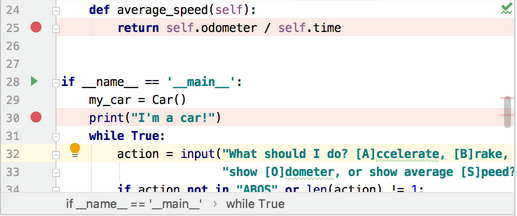
\includegraphics[scale = 0.4]{1}
\end{center}
\caption{Postavljanje tačaka prekida.}
\label{1}
\end{figure}
    
\end{frame}
\subsection{Opcije Debugger-a}
\begin{frame}{Opcije Debugger-a}
Sve opcije Debugger-a se nalaze u Debug Tool Window-u.\\
\textbf{Inline Debbuger} je opcija koja nam pruža da u vidu komentara u editoru vidimo sve vrednosti promenljivih.\\
\textbf{Evaluacija izraza} je opcija koja nam omogućava da izračunamo bilo koji izraz sa trenutnim vrednostima promenljivih u kodu, kao i da dodeljujemo vrednosti promenljivama.\\
\textbf{Posmatranja} su zaseban prozor u kome se nalaze sve promenljive koje su trenutno definisane, kao i njihove vrednosti.\\
\textbf{Detaljno debagovanje} predstavlja skup opcija za iteriranje kroz kod korak po korak.
\end{frame}

%------------------------------------------------
\section{Literatura}
\begin{frame}
\frametitle{Literatura}
\footnotesize{
\begin{thebibliography}{} % Beamer does not support BibTeX so references must be inserted manually as below
\bibitem[Kristian, 2017]{p1} Kristian Rother (2017)
\newblock Pro Python Best Practices Debugging, Testing and Maintenance

\bibitem[Adawadkar, 2017]{p2} Kalyani Adawadkar (2017)
\newblock Python Programming-Applications and Future
\newblock International Journal of Advance Engineering and Research Development

\bibitem[PythonDocs]{p3} Python 3.8.2 documentation
\newblock \url{https://docs.python.org/3/}

\bibitem[PyCharm]{p4} PyCharm
\newblock \url{https://www.jetbrains.com/help/pycharm/}
\end{thebibliography}
}

\end{frame}

%------------------------------------------------

%\begin{frame}
%\Huge{\centerline{Pitanja?}}
%\end{frame}

%----------------------------------------------------------------------------------------

\end{document} 
